\documentclass[11pt,a4paper]{article}

\usepackage[utf8]{inputenc}
\usepackage[T1]{fontenc}
\usepackage{geometry}
\usepackage{graphicx}
\usepackage{float}
\usepackage{xcolor}
\usepackage{listings}
\usepackage{tikz}
\usepackage{hyperref}
\usepackage{longtable}
\usepackage{array}
\usepackage{caption}

\geometry{margin=2.2cm}
\setlength{\parindent}{0pt}
\setlength{\parskip}{6pt}

\definecolor{codebg}{RGB}{245,245,245}
\lstset{
    basicstyle=\ttfamily\small,
    backgroundcolor=\color{codebg},
    breaklines=true,
    frame=single,
    columns=fullflexible
}

\newcommand{\terminalimage}[2]{
\begin{figure}[H]
    \centering
    \includegraphics[width=\textwidth,height=0.76\textheight,keepaspectratio]{\detokenize{#1}}
    \caption{#2}
\end{figure}
}

\begin{document}

\begin{titlepage}
    \centering
    \vspace*{2cm}
    {\Huge CSE 344 System Programming\par}
    \vspace{0.6cm}
    {\LARGE Homework 6 Report\par}
    \vspace{0.6cm}
    {\Large Magic Academy\par}
    \vfill
    \begin{tabular}{rl}
        Name: & Halit Batuhan Aslan \\
        Student ID: & 220104004003 \\
        Course: & CSE 344 System Programming \\
        Homework: & 6 \\
        Date: & 14 May 2026 \\
    \end{tabular}
    \vfill
\end{titlepage}

\tableofcontents
\newpage

\section{Introduction}

This homework implements a TCP based Magic Academy system in C. There are three separate programs:
\texttt{hogwarts}, \texttt{wizard}, and \texttt{professor}. The server accepts both wizard and professor
clients on the same TCP port. It uses \texttt{select()} for all connected clients, so there is no
thread-per-client model.

The implementation is split into small modules. The \texttt{hogwarts.c}, \texttt{wizard.c}, and
\texttt{professor.c} files only contain program entry points. Most server logic is moved to
\texttt{server.c}, \texttt{server\_clients.c}, \texttt{server\_protocol.c}, \texttt{server\_options.c},
and \texttt{server\_log.c}. Common socket and parsing helpers are in \texttt{common.c}. Ingredient
loading and snapshot creation are in \texttt{ingredients.c}. This made the code easier to test and
also keeps the three executable targets separate.

\section{System Design}

The server starts by parsing command line options, loading the ingredient file, opening the log file,
and creating one listening TCP socket. After this setup, the server enters one main event loop. This
loop manages both the listening socket and all client sockets with \texttt{select()}.

\begin{figure}[H]
\centering
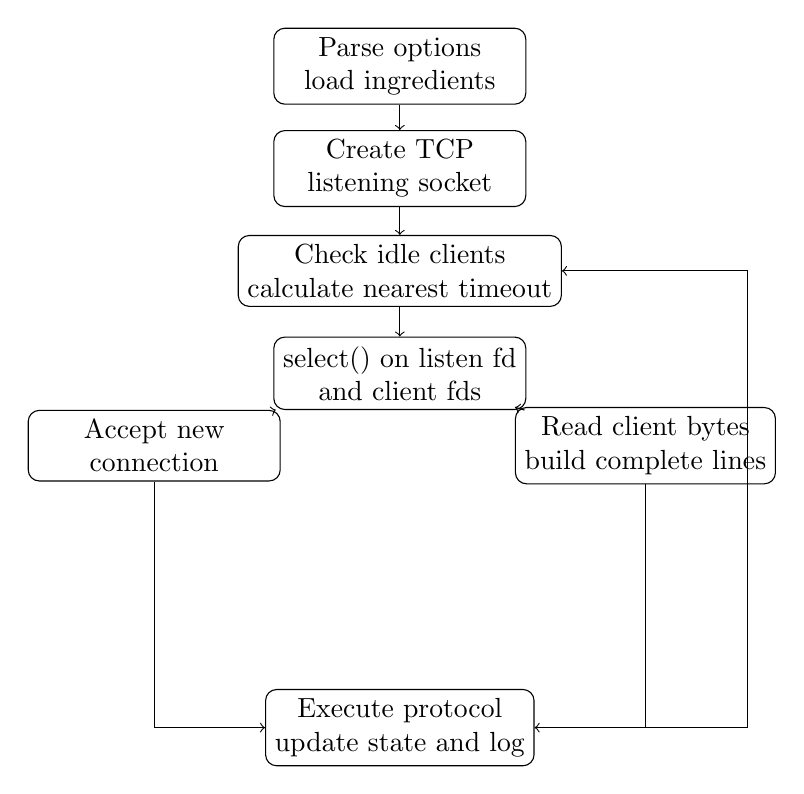
\begin{tikzpicture}[node distance=1.3cm, every node/.style={draw, rounded corners, align=center, minimum width=3.2cm, minimum height=0.8cm}]
    \node (start) {Parse options\\load ingredients};
    \node (listen) [below of=start] {Create TCP\\listening socket};
    \node (timeout) [below of=listen] {Check idle clients\\calculate nearest timeout};
    \node (select) [below of=timeout] {select() on listen fd\\and client fds};
    \node (accept) [below left of=select, xshift=-2.2cm] {Accept new\\connection};
    \node (client) [below right of=select, xshift=2.2cm] {Read client bytes\\build complete lines};
    \node (protocol) [below of=select, yshift=-3.2cm] {Execute protocol\\update state and log};
    \draw[->] (start) -- (listen);
    \draw[->] (listen) -- (timeout);
    \draw[->] (timeout) -- (select);
    \draw[->] (select) -- (accept);
    \draw[->] (select) -- (client);
    \draw[->] (accept) |- (protocol);
    \draw[->] (client) |- (protocol);
    \draw[->] (protocol.east) -- ++(2.7,0) |- (timeout.east);
\end{tikzpicture}
\caption{Single-threaded server loop}
\end{figure}

\subsection{No Thread Per Client}

The server does not create threads or child processes for clients. Each connected client has a record
inside the server context. The main loop rebuilds the \texttt{fd\_set} before every \texttt{select()}
call. If the listening socket is readable, the server calls \texttt{accept()}. If a client socket is
readable, the server reads bytes from that socket and processes complete protocol lines.

\subsection{Capacity Handling}

The maximum number of clients is given by \texttt{-n}. When this limit is reached, the server still
accepts the new TCP connection first. It immediately sends:

\begin{lstlisting}
ERR HOGWARTS_FULL
\end{lstlisting}

Then it logs the rejection and closes that new socket. This is done so the connecting client receives
a clear error instead of waiting silently.

\subsection{Idle Timeout Handling}

Every client stores \texttt{last\_active}. The server checks all clients before each \texttt{select()}
call. If a client has been inactive for at least the configured timeout, the server sends:

\begin{lstlisting}
TIMEOUT DISCONNECT
\end{lstlisting}

Then the client state is cleaned. For remaining clients, the server calculates the minimum remaining
time and passes it as the timeout argument to \texttt{select()}. Because of this, timeout control uses
no \texttt{sleep()} and no helper thread in the server.

\section{Program Structure}

\begin{longtable}{|p{4.1cm}|p{10.1cm}|}
\hline
\textbf{File} & \textbf{Responsibility} \\
\hline
\texttt{hogwarts.c} & Server executable entry point. Calls \texttt{run\_hogwarts\_server}. \\
\hline
\texttt{server.c / server.h} & Main server lifecycle, \texttt{select()} loop, timeout calculation, shutdown sequence. \\
\hline
\texttt{server\_types.h} & Shared server structs such as \texttt{client\_t}, \texttt{server\_options\_t}, and \texttt{server\_context\_t}. \\
\hline
\texttt{server\_clients.c / .h} & Listening socket, accepting clients, full server rejection, client cleanup. \\
\hline
\texttt{server\_protocol.c / .h} & Protocol commands: \texttt{ENROLL}, \texttt{BREW}, \texttt{CONSUME}, \texttt{SPELLBOOK}, \texttt{INSPECT}, \texttt{SCROLL}, \texttt{ROSTER}, \texttt{APPARATE}. \\
\hline
\texttt{server\_options.c / .h} & Command line parsing and usage message. \\
\hline
\texttt{server\_log.c / .h} & Timestamped server logging to stdout and the given log file. \\
\hline
\texttt{wizard.c} & Wizard executable entry point. \\
\hline
\texttt{professor.c} & Professor executable entry point. \\
\hline
\texttt{client\_app.c / .h} & Shared TCP client loop used by both wizard and professor. \\
\hline
\texttt{common.c / .h} & Shared helpers for sending complete lines, parsing numbers, splitting commands. \\
\hline
\texttt{ingredients.c / .h} & Ingredient table loading, lookup, scroll snapshot, spellbook snapshot. \\
\hline
\end{longtable}

\section{Data Structures}

The most important server-side structure is \texttt{client\_t}. It stores all per-client state.

\begin{lstlisting}[language=C]
typedef struct
{
    int fd;
    char username[MAX_USERNAME_LENGTH + 1];
    char type[MAX_TYPE_LENGTH + 1];
    char line_buf[MAX_LINE_LENGTH];
    size_t line_len;
    int line_too_long;
    time_t last_active;
    long *spellbook;
} client_t;
\end{lstlisting}

The spellbook is a \texttt{long} array. It has the same order and size as the global ingredient table.
For example, if \texttt{MOONSTONE} is at index 0 in the global ingredient table, the wizard's amount of
\texttt{MOONSTONE} is stored at \texttt{spellbook[0]}. This avoids another map structure and is simple
for this homework.

The global ingredient list is stored in \texttt{ingredient\_table\_t}. Invalid ingredient file lines are
skipped silently as required. Duplicate ingredient names are also skipped.

\begin{figure}[H]
\centering
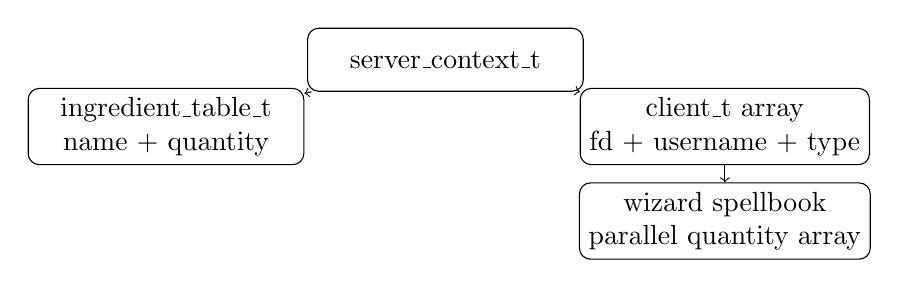
\begin{tikzpicture}[node distance=1.2cm, every node/.style={draw, rounded corners, align=center, minimum width=3.5cm, minimum height=0.8cm}]
    \node (context) {server\_context\_t};
    \node (ingredients) [below left of=context, xshift=-2.7cm] {ingredient\_table\_t\\name + quantity};
    \node (clients) [below right of=context, xshift=2.7cm] {client\_t array\\fd + username + type};
    \node (book) [below of=clients] {wizard spellbook\\parallel quantity array};
    \draw[->] (context) -- (ingredients);
    \draw[->] (context) -- (clients);
    \draw[->] (clients) -- (book);
\end{tikzpicture}
\caption{Main server data ownership}
\end{figure}

\section{Protocol Handling}

The server requires \texttt{ENROLL} as the first command. If a client sends any other command before
enrolling, the server responds with:

\begin{lstlisting}
ERR NOT_ENROLLED
\end{lstlisting}

After enrollment, the server uses the stored client type to authorize commands. Wizards can use
\texttt{BREW}, \texttt{CONSUME}, and \texttt{SPELLBOOK}. Professors can use \texttt{INSPECT},
\texttt{SCROLL}, and \texttt{ROSTER}. If a professor sends \texttt{BREW} or \texttt{CONSUME}, the
server returns \texttt{ERR UNAUTHORIZED}. The same authorization rule is applied when a wizard tries
professor commands.

\subsection{Ingredient Updates}

\texttt{BREW} increases both the global ingredient quantity and the wizard's spellbook quantity.
\texttt{CONSUME} decreases both, but only if the global stock and the wizard's own spellbook have
enough amount. The global quantity never becomes negative.

\section{Partial Read and Write Handling}

TCP does not preserve message boundaries. Because of that, the server stores incoming bytes in
\texttt{line\_buf}. When a newline is received, that complete line is parsed. If more than 511 useful
characters arrive before newline, \texttt{line\_too\_long} is marked and the server answers
\texttt{ERR TOOLONG} when the newline is reached.

Outgoing messages use \texttt{send\_all}. It keeps calling \texttt{send()} until all bytes are written.
This is needed because \texttt{send()} may write only part of a message.

\section{Signal Handling and Shutdown}

The server and clients install a \texttt{SIGINT} handler. The handler only sets a
\texttt{volatile sig\_atomic\_t} flag. The real shutdown logic happens in the normal control flow.

\begin{figure}[H]
\centering
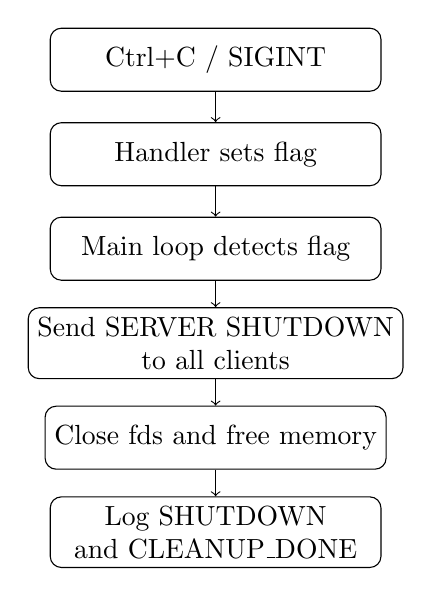
\begin{tikzpicture}[node distance=1.2cm, every node/.style={draw, rounded corners, align=center, minimum width=4.2cm, minimum height=0.8cm}]
    \node (sig) {Ctrl+C / SIGINT};
    \node (flag) [below of=sig] {Handler sets flag};
    \node (loop) [below of=flag] {Main loop detects flag};
    \node (notice) [below of=loop] {Send SERVER SHUTDOWN\\to all clients};
    \node (close) [below of=notice] {Close fds and free memory};
    \node (log) [below of=close] {Log SHUTDOWN\\and CLEANUP\_DONE};
    \draw[->] (sig) -- (flag);
    \draw[->] (flag) -- (loop);
    \draw[->] (loop) -- (notice);
    \draw[->] (notice) -- (close);
    \draw[->] (close) -- (log);
\end{tikzpicture}
\caption{Server shutdown sequence}
\end{figure}

For wizard and professor clients, Ctrl+C causes the main loop to send \texttt{APPARATE}. The client
then waits for \texttt{OK APPARATE} or a shutdown/timeout notice, closes the socket, and exits.

\section{Output Format}

Server log lines use the required prefix style with timestamps:

\begin{lstlisting}
[2026-05-14 21:47:00] [SERVER] CLEANUP_DONE clients=0
\end{lstlisting}

Client outputs use:

\begin{lstlisting}
[WIZARD harry] RECEIVED OK SPELLBOOK MOONSTONE:10
[PROFESSOR mcgonagall] RECEIVED ERR UNAUTHORIZED
\end{lstlisting}

The assignment examples show some client lines without the bracket prefix, but the output keyword
table says the prefix is mandatory. So I used the stricter table format.

\section{Build Result}

\terminalimage{report_assets/build_terminal.png}{Build output with gcc flags and make clean}

\section{Mandatory Test Scenarios}

The following figures are uncut terminal screenshots taken during the mandatory scenario runs. Each
scenario was started with a fresh server, and the screenshots show the commands and the program
outputs from start to finish.

\subsection{Scenario 1}

This scenario checks duplicate username, command before \texttt{ENROLL}, unknown wizard command,
unauthorized professor commands, unauthorized wizard professor-commands, and normal disconnect.

\terminalimage{report_assets/scenario1_server.png}{Scenario 1 server terminal and log}
\terminalimage{report_assets/scenario1_wizard_hermione.png}{Scenario 1 wizard Hermione terminal}
\terminalimage{report_assets/scenario1_duplicate_hermione.png}{Scenario 1 duplicate Hermione terminal}
\terminalimage{report_assets/scenario1_not_enrolled_client.png}{Scenario 1 raw client before ENROLL}
\terminalimage{report_assets/scenario1_professor_dumbledore.png}{Scenario 1 professor Dumbledore terminal}

\subsection{Scenario 2}

This scenario checks ingredient updates, spellbook tracking, insufficient own spellbook amount,
unknown ingredient, scroll snapshot, roster, and professor inspect.

\terminalimage{report_assets/scenario2_server.png}{Scenario 2 server terminal and log}
\terminalimage{report_assets/scenario2_wizard_harry.png}{Scenario 2 wizard Harry terminal}
\terminalimage{report_assets/scenario2_professor_mcgonagall.png}{Scenario 2 professor McGonagall terminal}

\subsection{Scenario 3}

This scenario checks maximum capacity, rejection recovery after a client leaves, and roster after a
new client connects.

\terminalimage{report_assets/scenario3_server.png}{Scenario 3 server terminal and log}
\terminalimage{report_assets/scenario3_wizard_harry.png}{Scenario 3 wizard Harry terminal}
\terminalimage{report_assets/scenario3_wizard_ron.png}{Scenario 3 wizard Ron terminal}
\terminalimage{report_assets/scenario3_professor_dumbledore.png}{Scenario 3 professor Dumbledore terminal}
\terminalimage{report_assets/scenario3_wizard_voldemort.png}{Scenario 3 rejected wizard Voldemort terminal}
\terminalimage{report_assets/scenario3_professor_snape.png}{Scenario 3 rejected professor Snape terminal}
\terminalimage{report_assets/scenario3_wizard_neville.png}{Scenario 3 wizard Neville terminal}

\subsection{Scenario 4}

This scenario checks idle timeout, continuing activity for another wizard, later client joins,
professor queries, server Ctrl+C, and process cleanup.

\terminalimage{report_assets/scenario4_server.png}{Scenario 4 server terminal and log}
\terminalimage{report_assets/scenario4_wizard_hermione.png}{Scenario 4 active wizard Hermione terminal}
\terminalimage{report_assets/scenario4_wizard_harry_idle.png}{Scenario 4 idle wizard Harry timeout terminal}
\terminalimage{report_assets/scenario4_wizard_ron.png}{Scenario 4 wizard Ron terminal}
\terminalimage{report_assets/scenario4_professor_dumbledore.png}{Scenario 4 professor Dumbledore terminal}
\terminalimage{report_assets/scenario4_professor_mcgonagall.png}{Scenario 4 professor McGonagall terminal}

\section{Challenges}

\subsection{Handling TCP Lines Correctly}

The first important issue was that TCP can split one command into multiple reads or join many commands
in one read. So I did not parse directly after every \texttt{recv()}. Instead, every client has a
line buffer. Bytes are appended until newline. This fixed partial reads and also made \texttt{ERR
TOOLONG} easier to implement.

\subsection{Idle Timeout Without Sleep}

Another problem was idle timeout. A simple \texttt{sleep()} loop would break the homework rule and
also block client processing. I solved it by checking clients before every \texttt{select()} call and
calculating the nearest remaining timeout. This lets \texttt{select()} wake up exactly when the next
client may timeout.

\subsection{Shared Client Code}

Wizard and professor clients are very similar, but their role names are different. I moved the common
client logic into \texttt{client\_app.c}. This avoided duplicated socket and signal handling code.
The server still enforces the actual permissions, so the professor program cannot bypass rules.

\section{Conclusion}

The final implementation builds three programs with the required compiler flags. The server uses one
\texttt{select()} loop, maintains per-client state, rejects extra clients when full, disconnects idle
clients, handles Ctrl+C cleanly, and implements the required protocol responses. The mandatory
scenario outputs show the main behavior expected by the homework.

\end{document}
